%%%%%%%%%%%%%%%%%%%%%%%%%%%%%%%%%%%%%%%%%%%%%%%%%%%%%%%%%%%%%%%%%%%%%%%%
% QE_notes - Notes about the simulation of the QE of PMTs
%
% Filename: $RCSfile$
% Author:   $Author$
% Revision: $Revision$
% Date:     $Date$
%%%%%%%%%%%%%%%%%%%%%%%%%%%%%%%%%%%%%%%%%%%%%%%%%%%%%%%%%%%%%%%%%%%%%%%%

\documentclass{article}

\usepackage{a4wide}
\usepackage{amstext}
\usepackage{amsmath}
\usepackage{epsfig}
\usepackage{xspace}

\def\Cherenkov{Cherenkov\xspace}

\def\cph{Ch.\ensuremath{\gamma}\xspace}
\def\cphs{Ch.\ensuremath{\gamma}s\xspace}

\def\phe{ph.e\ensuremath{^{-}}\xspace}
\def\phes{ph.e\ensuremath{^{-}}s\xspace} 

\def\QE{\ensuremath{\mathcal{QE}}\xspace}

\def\Nphot{\ensuremath{%
  \mathcal{N}_{\gamma}}\xspace}
\def\Ntrial{\ensuremath{%
  \mathcal{N}_{\mathrm{ph.e.s}}}\xspace}
\def\Nmean{\ensuremath{%
  \bar\mathcal{N}_{\mathrm{ph.e.s}}}\xspace}
\def\Nrand{\ensuremath{%
  \mathcal{N}^{\mathrm{r}}_{\mathrm{ph.e.s}}}\xspace}
\def\Ntrialrand{\ensuremath{%
  \mathcal{N}^{\mathrm{t+r}}_{\mathrm{ph.e.s}}}\xspace}


%%% BEGIN %%%%%%%%%%%%%%%%%%%%%%%%%%%%%%%%%%%%%%%%%%%%%%%%%%%%%%%%%%%%

\begin{document}

\begin{center}
  {\large \scshape 
  Notes on the simulation of the response of a photomultiplier tube\\}
  J. C. Gonz\'alez\\
  {\small Max-Planck-Institut f\"ur Physik, 
  F\"ohringer Ring 6, D-80805 M\"unchen, Deutschland\\
  E.mail: \texttt{gonzalez@mppmu.mpg.de}\\}
  January, 2000
\end{center}

%------------------------------------------------------------

\begin{abstract}
  The simulation of the response of a photomultiplier tube (PMT) can
  be performed with a simple procedure, despite of its complexity. One
  just has to have very clear the nature of the whole process, step by
  step. In this small notes I try to clarify the physical processes
  involved.
\end{abstract}

%------------------------------------------------------------

\section*{Introduction}

The simulation of the response of a photomultiplier tube (PMT) can be
performed with a simple procedure, despite of the complexity of the
process. These notes are written down simply to clarify the effects
that have to be taken into account, like the Quantum Efficiency (QE)
of the PMT (usually a function of the wavelength of the incident
photon $\gamma$), the natural fluctuations of this QE for a given
fixed wavelength, the first dynode response, the possible
afterpulsing, the single photoelectron response of the PMT, etc. In
this small note I will try to clarify some concepts about the
simulation of the conversion of normal photons (in our case of
\Cherenkov astronomy, \Cherenkov photons and photons coming from the
Light of Night Sky and starlight) into number of photoelectrons after
the photocathode.

%------------------------------------------------------------

\section{Fluctuations taking place}

Before we try to understand this process of conversion of \Cherenkov
photons into photoelectrons, let's try to identify the possible
sources of fluctuations.

In the first place, we have a given number of incoming \Cherenkov
photons, which fluctuates. This is due to the statistical nature of
the generation of the atmospheric shower. This means that even for a
fixed energy of the primary particle which generated the shower, the
probabilistic generation of secondary particles, the fluctuations in
the height of the first interaction (and hence in the height where the
maximum particle generation is achieved) and the random generation of
\Cherenkov photons by charged particles will lead to a fluctuating
number of Cherenkov photons.

At the end of the cascading process, and after we introduce the
simulation any given set of reflecting or guiding devices in our
instrument, we will have an input number of photons in the
photomultiplier tube. I will call this number of photons \Nphot.

Now we want to simulate a measurement of \Nphot leading to a certain
current I, or a given amount of electrons in the anode
$N_{\mathrm{e}}$. The \Cherenkov photons hitting the photocathode will
produce a given number of photoelectrons. This process is
probabilistic, and depends on the QE of the photocathode. But this QE
not only depends of the wavelength of the incident photon. It also
depends on the specific place of the photocathode where the photon
hits. Additionally, the measured QE of a PMT is just an average value
over many photons. This means that the QE itself must be seen as a
fluctuating term, in the sense of its probabilistic nature.

%\begin{figure}[tb]
%  \begin{center}
%    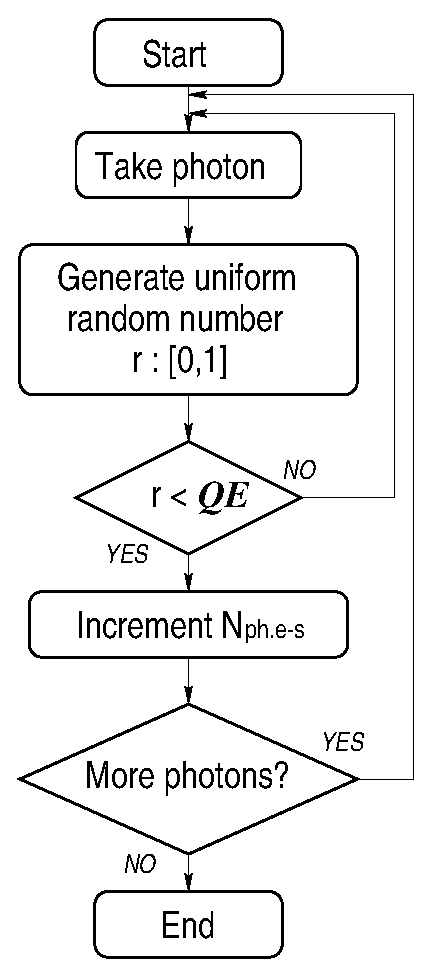
\epsfig{file=qefig1bis.eps,width=0.25\textwidth}
%    \caption{Simple algorithm to simulate the conversion of incoming
%      photons into photoelectrons in a photocathode with a given Quantum
%      Efficiency \QE.}
%    \label{fig:algorithm1}
%  \end{center}
%\end{figure}

After the photoelectrons are emitted from the photocathode, a certain
number of them will arrive at the first dynode. Of course, this
depends on the place where the photoelectron come from, and on the
design of the PMT itself. This is the so called \emph{first dynode
collection efficiency}. Different measurements lead to a value of
about 90\%. After hitting the first dynode, each photoelectron can
liberate a typical number of 6 electrons, but again this can
fluctuate. 

We just started the cascading process. After the first dynode comes
the second, where we again have a multiplicating term and an
efficiency term. This multiplicating process continues until we reach
the anode, where we finally have a big number of electrons, depending
on the gain and the voltage of our PMT.

Al this cascade process can be simulated by using the so called
\emph{single photoelectron response} or \emph{single electron
spectrum} (SES) of the photomultiplier, which is nothing but the
distribution of the output we get from the photomultiplier for a
single photoelectron release by the photocathode. This depends also on
the high voltage applied to the PMT. Therefore, by using this
distribution, we can simulate the output of each single photoelectron,
superpose all these output, and we will get at the end a realistic
view of the response of our PMT to the incident amount of light.

%------------------------------------------------------------

\section{Simulation of the Quantum Efficiency}

In this document we assume that \emph{a single photon cannot produce,
for whatever processes inside the photocathode, more than one
photoelectron}. For each single photon the generation of a
photoelectron is therefore what is called a \emph{Bernoulli} process:
we can have only two outcomes: success (with probability $p$), or fail
(with probability $1-p$). For a given number of incoming photons the
generation of photoelectrons is a good example of a \emph{binomial}
process. Let's first forget about the dependency of the Quantum
Efficiency with the wavelength. Let's assume, therefore, that we have
a monochromatic bunch of photons. We call then $\QE=$QE($\lambda_0$),
the Quantum Efficiency (the \emph{average} value, obtained by
measurements) of the photocathode at one fixed wavelength $\lambda_0$.

\begin{figure}[tb]
  \begin{center}
    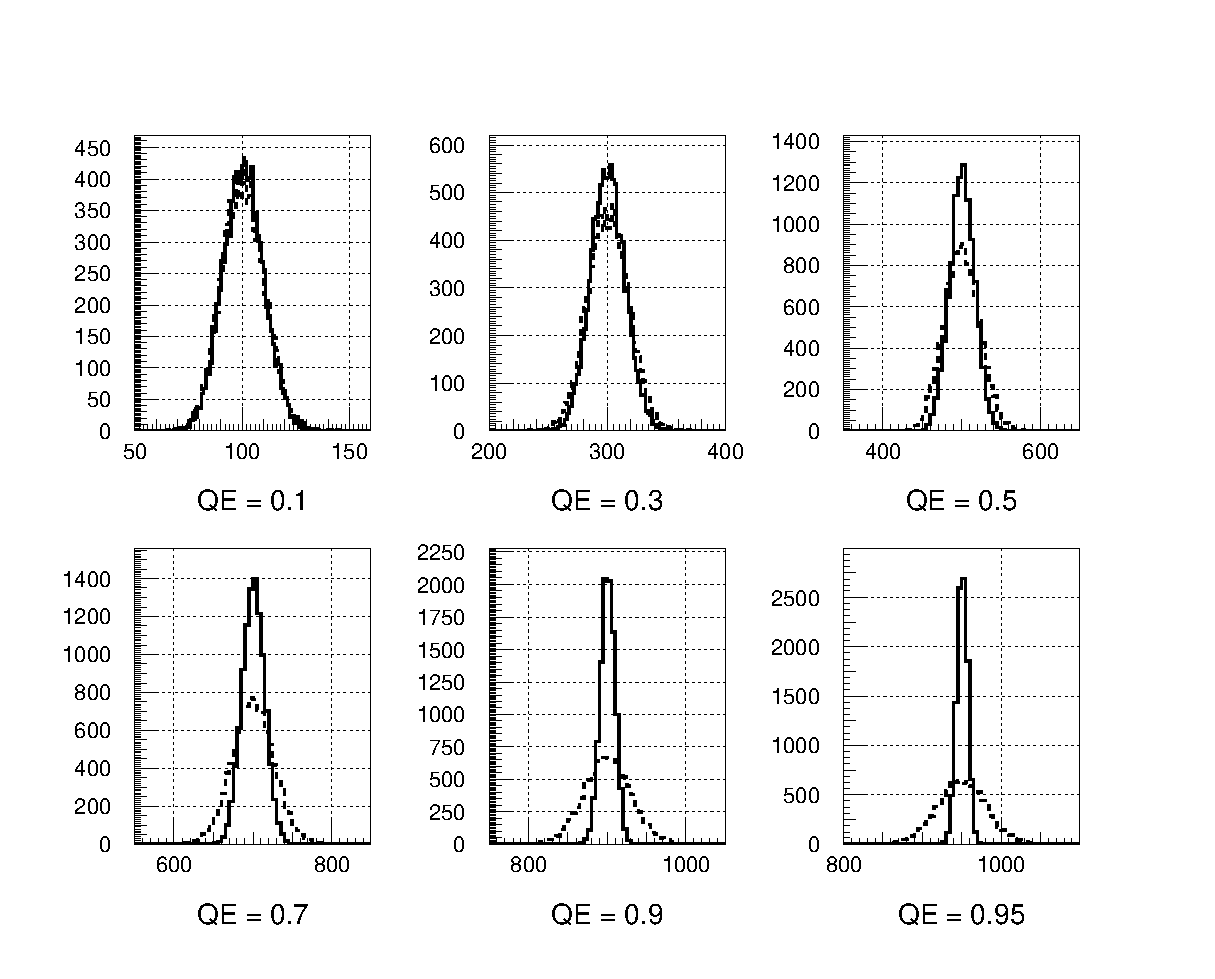
\epsfig{file=qehistqe.eps,width=0.8\textwidth}
    \caption[Distributions of the number of outcoming photoelectrons 
    for different QE.]{Distributions of the number of outcoming
      photoelectrons (\Ntrial, solid line; \Nrand, dashed line) for
      different values of \QE. In this case, $\Nphot=1000$.}
    \label{fig:distrib1}
  \end{center}
\end{figure}

We see that each incoming photon have a certain probability \QE of
generating a photoelectron. This can be simulated by using a
\emph{uniformly distributed random number} $X$ in the interval [0,1]
for each photon: whenever this number $X$ is smaller than \QE, we
assume the photon generated a photoelectron; otherwise, it didn't. A
simple algorithm to do this can is:

\begin{list}{}{}
\item[A1.] Take photon.
\item[A2.] Generate uniform random number $r$ in $(0,1)$.
\item[A3.] If $r < \QE$, take photon, else go to A1.
\item[A4.] Are there photons left? If yes, go to A1; else Stop.
\end{list}

Of course, after following this algorithm \Nphot times we will have,
\emph{on average}, a number of photoelectrons:

\begin{equation}
  \Nmean = \Nphot \times \QE
\end{equation}

The words \emph{on average} means simply that we will not get, from
our experiment, exactly a number \Nmean of photoelectrons. At least,
not always. If we repeat this experiment a lot of times we will get
instead a distribution of numbers \Ntrial, corresponding to the number
of photoelectrons produced. This distribution, given the
\emph{binomial} nature of the process, will result in a \emph{binomial
distribution}. The mathematical expresion for this is:

\begin{eqnarray}
  \mathcal{P}_{\mathrm{Binom}}(r)
  &=& \binom{N}{r} p^{r} q^{N-r} \\ 
  &=& \frac{N!}{r!(N-r)!} p^{r} (1-p)^{N-r} \nonumber
\end{eqnarray}

where $\mathcal{P}_{\mathrm{Binom}}(r)$ is the probability of getting
$r$ successes out of $N$ independent trial, each of which has only two
possible outcomes: success (with probability $p$) or failure (with
probability $q=1-p$). We can show that the expectation value of the
number of successes is $\bar{r}=\sum r\mathcal{P}(r) = Np$, which is
far for surprising. For this distribution we have also that
$\sigma^{2} \leq \bar{r}$, where the equality holds only for p=0. In
general the variance is smaller than the mean. This is so because the
upper limit imposed on $r$ (which cannot be larger than $N$) reduces
the spread of the $r$-distribution.

\begin{figure}[bt]
  \begin{center}
    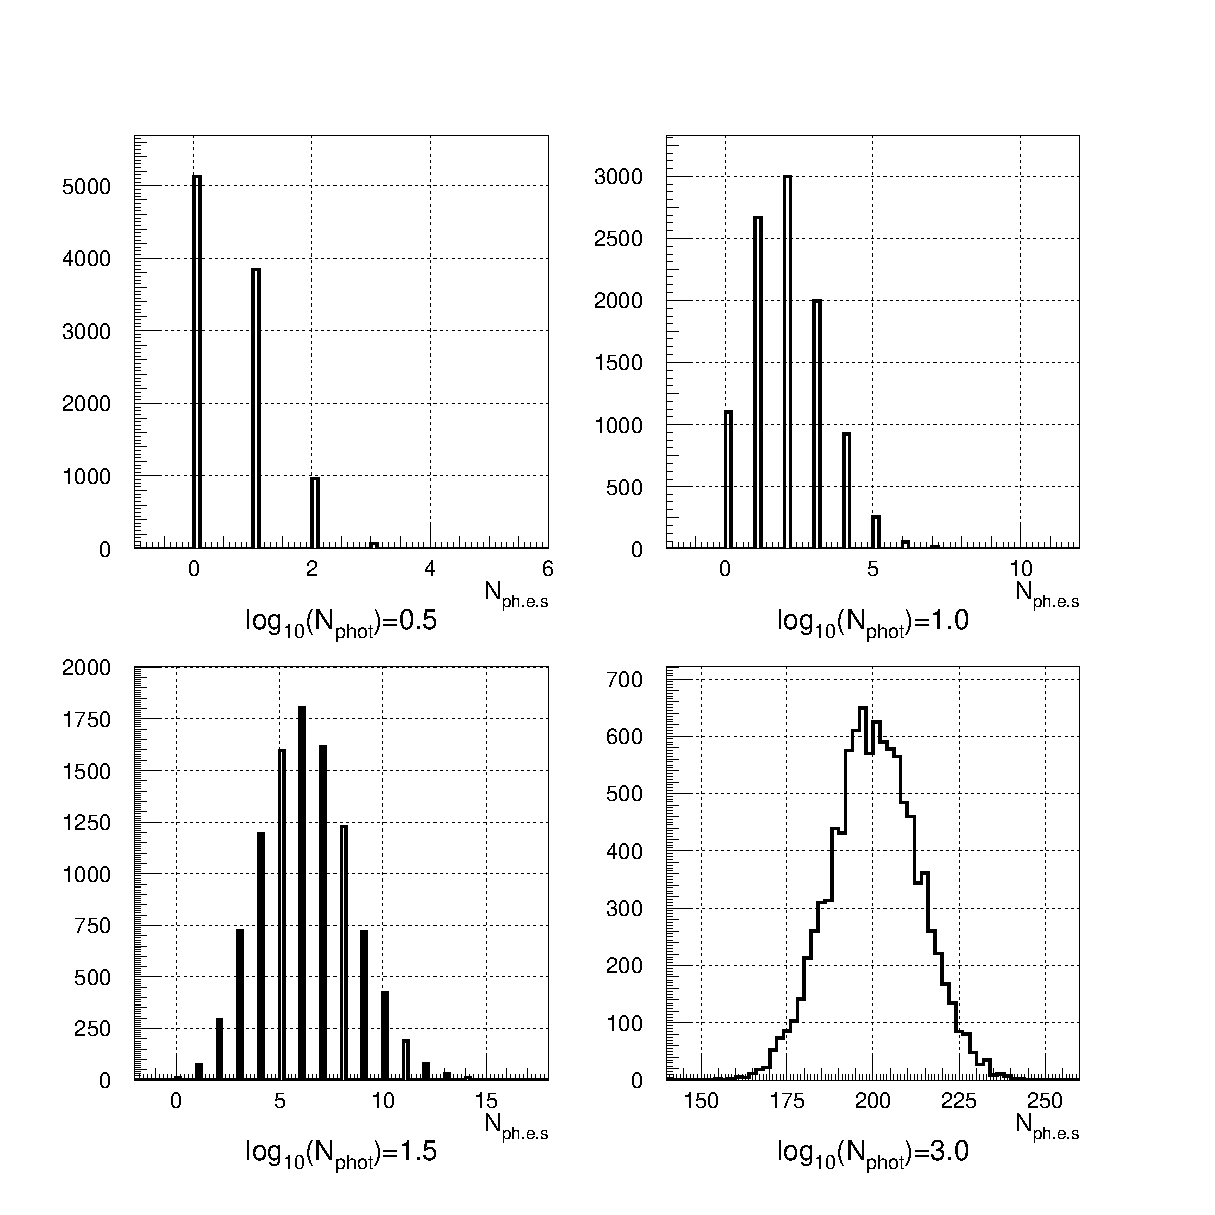
\epsfig{file=varwithp.eps,width=0.65\textwidth}
    \caption[Distributions of the number of outcoming photoelectrons 
    for different amount of incoming photons]{Distributions of the
      number of outcoming photoelectrons (\Ntrial) for different
      values of \Nphot (in these cases
      $\log_{10}\Nphot=0.5,1.0,1.5\text{ and }3.0$), using a
      $\QE=0.2$.}
    \label{fig:varwithp}
  \end{center}
\end{figure}

\begin{figure}[tb]
  \begin{center}
    \epsfig{file=varwithqe.eps,width=0.35\textwidth,angle=-90,clip=}
    \caption[Variation of z with different QE]{Variation with different 
      \QE of the quotient $z=\sigma(\Nrand)/\sigma(\Ntrial)$, also in
      the case of $\Nphot=1000$. For another values of \Nphot the
      curve is very similar.}
    \label{fig:varwithqe}
  \end{center}
\end{figure}

\begin{figure}[bt]
  \begin{center}
    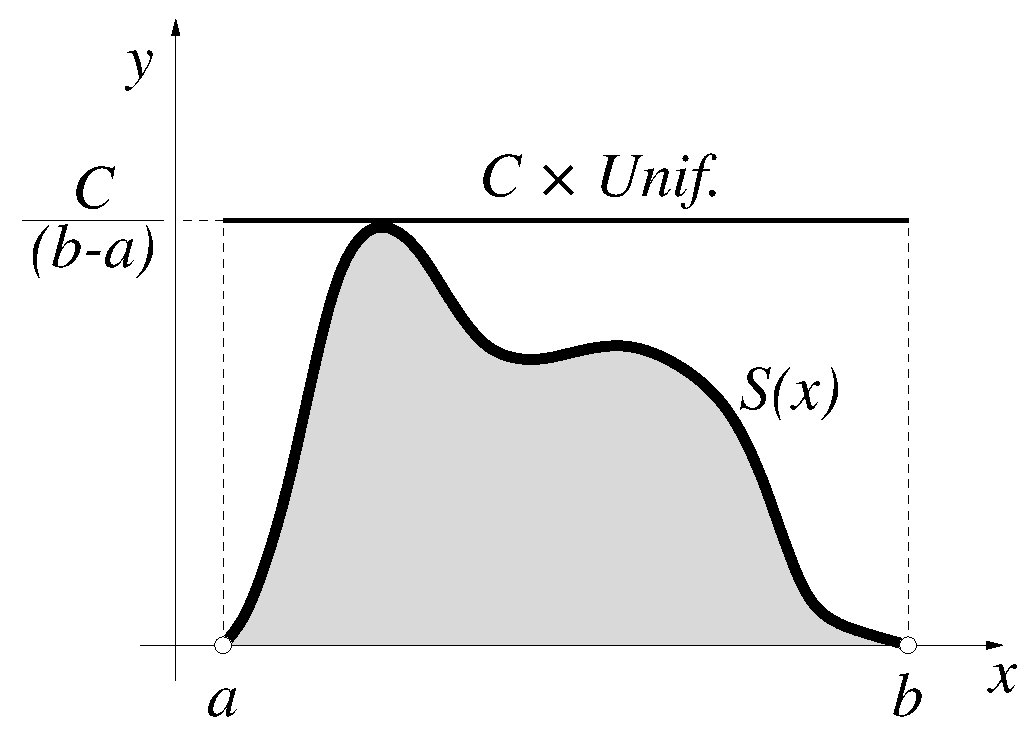
\epsfig{file=qefig2.eps,width=0.4\textwidth,clip=}
    \caption[Ilustration of the \emph{Acceptance-Rejection Method} (Von
      Neumann]{Ilustration of the \emph{Acceptance-Rejection Method} (Von
      Neumann). The pairs of random numbers $(x,y)$ will cover the
      area below the line $y=C/(b-a)$. Only those below the curve
      $S(x)$ will be accepted.}
    \label{fig:acceprejec} 
  \end{center} 
\end{figure}

The main use of the binomial distribution is in the limits:

\begin{enumerate}
\item $p\rightarrow 0$, $N\rightarrow\infty$, 
  but $Np=\mu$ (constant), when Binomial $\longrightarrow$ Poisson
\item $p=const.$, $N\rightarrow\infty$, 
  when Binomial $\longrightarrow$ Gaussian
\end{enumerate}

In our case, $N=\Nphot$, $p=\QE$ and $Np=\Nmean$.  This means that,
\emph{for \Nphot large and in the case of $\QE\rightarrow 0$} (more 
generally speaking, for \QE smal) the distribution of the number of
outcoming photoelectrons \Ntrial will be very similar to the
distribution obtained by using the mean number of photoelectrons
\Nmean as the mean value of a Poisson distribution. More clearly, 
the requierements of \Nphot large and \QE small are needed if we want
to use this procedure, what I will call the \emph{Poisson approach}.

The use of the \emph{Poisson approach} is very attractive because you
don't need to work with separate photons. Moreover, some times its the
most direct approach: you can get your photons at the entrance of the
PMT in bunches of several tens of photons. In this case it's more
comfortable to use mean values and the corresponding Poisson
distribution. We are sure that $N$ is going to be large enough. But we
still have to be sure that our \QE is small enough to allow us to use
this approach. Fortunately, this is normally the case.

\begin{figure}[bt]
  \begin{center}
    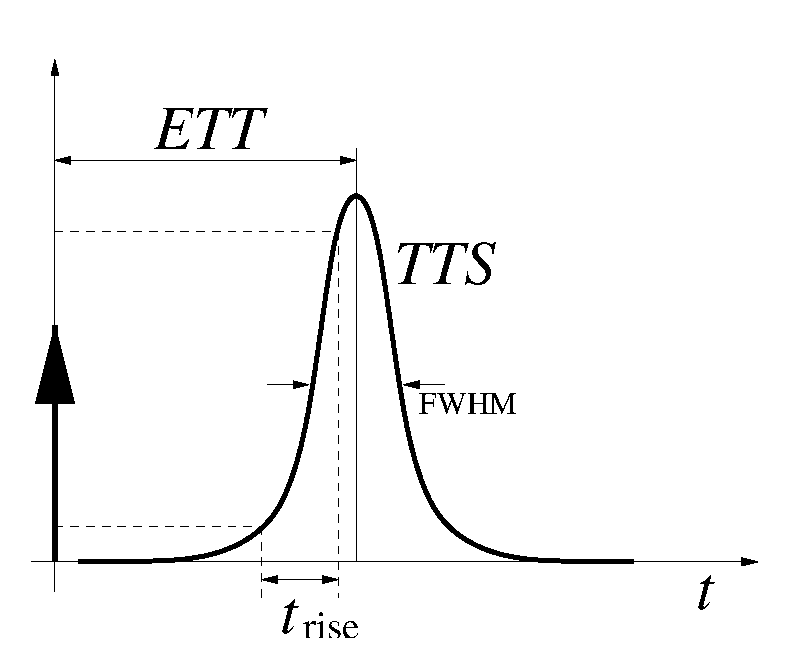
\epsfig{file=qefig3.eps,width=0.4\textwidth,clip=}
    \caption{Ilustration of the output signal for an incoming
      delta-function light pulse. The main parameters of the time 
      response of a PMT are shown.}
    \label{fig:timeresponse} 
  \end{center} 
\end{figure}

In order to show the possible deviations we can get by using the
\emph{Poisson approach}, A simple simulation was done, where a
pre-fixed number of photons \Nphot was sent to a hypothetic
photocathode, where we simulated the Bernoulli process of the
production of a photoelectron by using the simple algorithm before.
The \QE of the photocathode was also fixed, and we counted the number
of photoelectrons emerging from it \Ntrial.  In addition, using the
number of incoming photons and \QE, we estimated the average number of
photoelectrons \Nmean we should get, and then followed the
\emph{Poisson approach} to get the final number of photoelectrons
\Nrand.

In order to show how we can get severe deviations from the right
behavior by using the \emph{Poisson approach}, I performed the
simulation varying the number of incoming photons and the value of
\QE. The results are shown in Fig. \ref{fig:distrib1},
\ref{fig:varwithqe} \ref{fig:varwithp}. In Fig. \ref{fig:distrib1} we
see the effect of using a \QE very different from 0. For small values
of \QE, both distributions of photoelectrons \Ntrial (solid line) and
\Nrand (Dashed line) appear reasonably similar. However, as \QE is
diverging from our hypothesis of \QE small, both distributions get
more and more different. In Fig. \ref{fig:varwithqe} we can see how
different these distributions are for different \QE, by using the
quantity

\begin{equation}
  z=\frac{\sigma(\Nrand)}{\sigma(\Ntrial)}
\end{equation}

Although the mean value remains practically the same for both
distributions, no matter the value of \QE, the variance
$\sigma^2(\Nrand)$ increases much more than the variance
$\sigma^2(\Ntrial)$ with \QE increasing. As we said before, this is
just the result of the upper limit imposed in \Ntrial (it cannot be
larger than \Nphot).

%------------------------------------------------------------

\section{Simulation of Single Electron Spectrum}

This is just an application of the general procedure of getting a
series of random numbers following a user-defined distribution, called
the \emph{Acceptance-Rejection Method} (Von Neumann). Let's assume we
know the \emph{single electron spectrum}, $S(x)$, defined in an
interval $(a,b)$. This will be in principle a not normalized function
proportional to the normalized probability density function (p.d.f.)
of distribution we want to simulate. Then, choose a p.d.f. uniform on
the interval $(a,b)$. Find a constant $C$ such that $C$ times this
uniform p.d.f.  is everywhere $\geq S(x)$. The situation is shown in
Fig.  \ref{fig:acceprejec}. 

Then, first, simulate an $x$ uniformly on $(a,b)$. Then generate a $y$
on $(0,C/(b-a))$. The point $(x,y)$ will uniformly populate the box
shown. If $y\leq S(x)$, we accept $x$ as then next value f the random
number. If $y\geq S(x)$, reject $x$ and try again. This method is very
simple and has an efficiency (fraction of values $x$ accepted) of
$\epsilon = (\text{area under }S(x))/(\text{area under bounds})$.
(Note that if the function $S(x)$ has sharp peaks, the efficiency can
be very low; one can then use different constants for different
regions in the interval $(a,b)$.)

For each photoelectron we will get, by using this procedure, the
amplitude of the registered signal. In order to simulate a realistic
signal at the output of our PMT, we should use the arrival time of
each photon. On top of this time, the PMT introduces a delay. This
delay follows a distribution similar to a gaussian. The time between
the arrival of a delta-function light pulse and the time where the
output signal reaches its maximum is called \emph{electron transit
time} (ETT). The delay between our input light and the output signal
comes then governed by the ETT and the \emph{transit time spread}
(TTS, also called \emph{transit time jitter}, the FWHM of the
distribution of delays). The output signal is characterized by its
\emph{rise time} (time where the output signal rises from 10\% to
90\% of the maximum amplitude). Sometimes, instead of having the
\emph{rise time}, $t_{\mathrm{rise}}$ we have the FWHM of the output 
characteristic, $\approx 2.36\sigma$. The situation is schematized in
Fig. \ref{fig:timeresponse}. With all this we can reproduce
the response of our PMT to the to the bunch of incident photons.

After all this chain of events, we can then introduce either the
trigger logic of our system, or any electronic device which modifies
this signal.

\begin{thebibliography}{99}
  
\bibitem{statmeth} Eadie, W.T., et al., \emph{Statistical Methods in
    Experimental Physics}, North-Holland Publishing Company, 1971.
  
\bibitem{electront} Electron Tubes Ltd., \emph{Photomultipliers and
    Accesories}, 1996

\bibitem{hamamatsu} Hamamatsu Photonics K.K, \emph{Photomultiplier
    Tubes and Assemblies for Scintillation Counting \& High Energy
    Phisics}, TPMO0001E05, May 1998.

\bibitem{lectures} Yost, G.P, \emph{Lectures on Probability and
    Statistics}, LBL-16993 Rev., 84/HENP/3, University of California,
    June 1985.

\end{thebibliography}
\end{document}

%%% END

%%%%%%%%%%%%%%%%%%%%%%%%%%%%%%%%%%%%%%%%%%%%%%%%%%%%%%%%%%%%%% 
% Last log: $Log$
% Last log: Revision 1.2  2000/01/27 12:56:06  gonzalez
% Last log: *** empty log message ***
% Last log:
% Last log: Revision 1.1  2000/01/26 18:54:24  gonzalez
% Last log: *** empty log message ***
% Last log:
% Last log: Revision 1.1  2000/01/24 08:40:13  gonzalez
% Last log: QE_notes almost finished...
% Last log: 
% Last log: Revision 1.1 2000/01/21 17:33:12 gonzalez 
% Last log: Small document about simulation of QE in PMTs 
% Last log: 
%%EOF

